\documentclass[sigconf,natbib=false]{acmart}

%% =========================================================
%% Packages
%% =========================================================

% BibLaTeX
\RequirePackage[
    datamodel=acmdatamodel,
    style=acmnumeric
]{biblatex}

% Korean support
\usepackage{kotex}

% Math packages
\usepackage{amsmath}
\usepackage{amssymb}
\usepackage{mathtools}

% Table / figure utilities
\usepackage{booktabs}
\usepackage{adjustbox}
\usepackage{tikz}
\usetikzlibrary{arrows.meta, positioning}

%% =========================================================
%% Bibliography
%% =========================================================

\addbibresource{sample-base.bib}

%% =========================================================
%% ACM Copyright / Conference Information
%% =========================================================

\setcopyright{acmlicensed}

\copyrightyear{2026}
\acmYear{2026}

\acmDOI{XXXXXXX.XXXXXXX}

\acmConference[
    ICAIF '26
]{7th ACM International Conference on AI in Finance}{
    November 2026
}{Milan, Italy}

\acmISBN{978-1-4503-XXXX-X/26/11}

\begin{document}

%% 논문 제목
\title{QuantDiffusion: Multivariate Financial Scenario Generation for Portfolio Risk Assessment via Realized Volatility Decomposition}

%% 저자 정보 설정
\author{Juhwan Kim}
\orcid{0009-0001-0818-8912}
\affiliation{%
  \institution{Hanyang University}
  \city{Seoul}
  \country{Republic of Korea}
}
\email{juhwankim@hanyang.ac.kr}

\author{Soobeen Kim}
\affiliation{%
  \institution{Hanyang University}
  \city{Seoul}
  \country{Republic of Korea}
}

\author{JaeWook Song}
\authornote{Corresponding author.}
\affiliation{%
  \institution{Hanyang University}
  \city{Seoul}
  \country{Republic of Korea}
}

%% 상단 헤더 저자 표시 (Kim et al.)
\renewcommand{\shortauthors}{Kim et al.}

%%
%% The abstract is a short summary of the work to be presented in the
%% article.
\begin{abstract}
Various approaches, notably GANs, have been explored for synthesizing multivariate financial time series; although GANs capture stylized facts and cross asset dependence well, they admit no SDE based or probabilistic characterization and therefore lack interpretability. Diffusion models can remedy this shortcoming and have become the dominant paradigm for time series generation outside finance, yet existing diffusion models still fail to reproduce the stylized facts of returns faithfully and, due to the nature of diffusion training, struggle to model ordinary and tail events simultaneously. To address these limitations, we introduce QuantDiffusion. Guided by an analysis of the diffusion training process as Langevin dynamics, we normalize multivariate financial series through a realized volatility decomposition together with a Lambert~$W$ Gaussianization, and we adopt a dilated convolutional backbone with parallel large and small kernel branches to capture local and long horizon dependencies jointly. We find empirically that isolating the extreme mass of returns in this way is what allows ordinary and tail events to be learned simultaneously, and we show that the resulting design admits a consistent stochastic differential equation interpretation, which identifies a stochastic volatility jump diffusion as the process underlying the data a posteriori rather than as an assumption imposed at the outset. On real daily return data spanning equities, indices, and commodities, QuantDiffusion consistently improves upon state of the art baselines along three complementary dimensions: cross sectional dependence among assets, marginal return distributions across multiple horizons, and the nonlinear temporal dependence associated with volatility clustering. More importantly, it markedly reduces estimation errors in portfolio level tail risk measures, namely Value at Risk and Expected Shortfall, across diverse trading strategies, underscoring its applicability to scenario generation, stress testing, and other risk sensitive financial tasks.
\end{abstract}




%%
%% The code below is generated by the tool at http://dl.acm.org/ccs.cfm.
%% Please copy and paste the code instead of the example below.
%%
\begin{CCSXML}
<ccs2012>
 <concept>
  <concept_id>00000000.0000000.0000000</concept_id>
  <concept_desc>Do Not Use This Code, Generate the Correct Terms for Your Paper</concept_desc>
  <concept_significance>500</concept_significance>
 </concept>
 <concept>
  <concept_id>00000000.00000000.00000000</concept_id>
  <concept_desc>Do Not Use This Code, Generate the Correct Terms for Your Paper</concept_desc>
  <concept_significance>300</concept_significance>
 </concept>
 <concept>
  <concept_id>00000000.00000000.00000000</concept_id>
  <concept_desc>Do Not Use This Code, Generate the Correct Terms for Your Paper</concept_desc>
  <concept_significance>100</concept_significance>
 </concept>
 <concept>
  <concept_id>00000000.00000000.00000000</concept_id>
  <concept_desc>Do Not Use This Code, Generate the Correct Terms for Your Paper</concept_desc>
  <concept_significance>100</concept_significance>
 </concept>
</ccs2012>
\end{CCSXML}

\ccsdesc[500]{Do Not Use This Code~Generate the Correct Terms for Your Paper}
\ccsdesc[300]{Do Not Use This Code~Generate the Correct Terms for Your Paper}
\ccsdesc{Do Not Use This Code~Generate the Correct Terms for Your Paper}
\ccsdesc[100]{Do Not Use This Code~Generate the Correct Terms for Your Paper}

%%
%% Keywords. The author(s) should pick words that accurately describe
%% the work being presented. Separate the keywords with commas.
\keywords{scenario simulation, generative models, denoising diffusion probabilistic models, multivariate time series, expected shortfall, value at risk, langevin dynamics, volatility decomposition}

\received{20 February 2007}
\received[revised]{12 March 2009}
\received[accepted]{5 June 2009}

%%
%% This command processes the author and affiliation and title
%% information and builds the first part of the formatted document.
\maketitle
\section{INTRODUCTION}

% Necessity of time-series generation
The generation of financial time series plays a central role in modern quantitative finance, supporting applications such as trading strategy development, stress testing, and risk management~\cite{chan2015simulation, glasserman2004monte, taylor2008modelling}. Market simulators allow practitioners to explore adverse scenarios, quantify tail risk exposure, and evaluate portfolio decisions under shifting conditions; when they fail to capture the statistical and dependence structure of real markets, however, loss estimation becomes biased and portfolio risk assessment is distorted~\cite{Cont26}. The recently emerging field of deep hedging has further heightened the importance of underlying asset path generation, since a non parametrically trained hedger must be exposed to realistic dynamics together with a sufficiently rich set of tail scenarios~\cite{buehler2021deep}.

\subsection{Related Work}

% Limitations of traditional models
Traditional approaches to financial time series simulation rely on parametric models such as autoregressive (AR) processes~\cite{AR-model-2005}, GARCH models~\cite{GARCH}, and continuous time SDEs~\cite{SDE-1998}. While interpretable and widely used, their flexibility is limited when capturing the distributional asymmetry, nonlinear dependence, and high dimensional interactions of real markets, especially in the multivariate setting. Interest in non parametric generative models has grown against this backdrop.

% GAN-based models
Generative adversarial networks (GANs)~\cite{GAN} are the most representative non parametric generative models for time series generation and can represent complex distributions directly from data~\cite{GAN_simulation_1, GAN_simulation_2, GAN_simulation_3}. Their application to financial data, however, is complicated by volatility clustering, fat tails, and non stationarity, and various tailored designs have been proposed in response. COSCI-GAN~\cite{COSCI-GAN} preserves cross variable correlations through a central discriminator; SigCWGAN~\cite{SigCWGAN} combines an autoregressive structure with the path signature to model conditional future distributions; and Market-GAN~\cite{Market-GAN} conditions generation on market context information. FIN-GAN~\cite{fin-gan} specializes a standard GAN architecture for financial data, while QuantGAN~\cite{QuantGAN} uses a temporal convolutional network (TCN) backbone and the invertible Lambert--$W$ transform to Gaussianize fat tailed returns; the latter provides important inspiration for the present study. Tail-GAN~\cite{Cont26} additionally targets tail risk fidelity and notes that, because generative models are typically trained to minimize average error, the low frequency tail region remains comparatively hard to model.

Despite their effectiveness in reproducing stylized facts, GAN based generators offer no explicit interpretation in terms of stochastic processes or SDEs, and thus lack theoretical interpretability of the generated paths. Diffusion based generative models have recently attracted attention as a promising alternative.

% Diffusion-based models
Most diffusion based time series models build directly on developments originating in computer vision, so we briefly review these foundations before turning to time series specific designs. The denoising diffusion probabilistic model (DDPM)~\cite{DDPMHo20} suffers from inflated negative log likelihood (NLL) at later stages of the forward process, where the noised state is hard to distinguish from the original data. To mitigate this, the Latent Diffusion Model (LDM)~\cite{LDMRombach22} performs diffusion in a low dimensional latent space from which perceptually irrelevant details have been removed by an autoencoder, allowing the model to concentrate its capacity on the essential semantic structure. Pushing the idea further, the NDM~\cite{NDMBartosh23} replaces the simple Markov forward chain with a data dependent non Markovian latent sequence, in which a time dependent nonlinear map $F_\phi(x,t)$ actively reduces the data to a learnable form. A common thread is that, when the data distribution is complex, diffusion on a transformed, simplified representation outperforms diffusion on the raw observations a perspective that becomes essential in the financial setting.

This insight has motivated a parallel line of work in time series that simplifies the learning target via explicit decomposition. Diffusion-TS~\cite{DiffusionTSYuan24} embeds a trend seasonality residual decomposition into a transformer based diffusion framework with a Fourier based loss. PaD-TS~\cite{PaDTSLi25} combines population aware training with a dual channel transformer to address distribution shift and preserve population level statistics such as cross correlations. DDM-TS~\cite{DDMTSKim24} decomposes a multivariate series into trend and seasonality components via STL, trains a dedicated diffusion model on each, and fuses them through an adaptive gating module to minimize inter component interference. As DDM-TS points out, processing all components simultaneously within a single framework induces structural interference that damages temporal dependencies. The present study interprets, from an SDE perspective, why such decomposition is required during diffusion training, but in contrast to prior work it adopts a decomposition based on \emph{realized volatility}; the justification is developed in subsequent sections.

% TCN
The decomposition above determines \emph{what} the diffusion model should learn a Gaussianized standardized shock component and a separately modeled volatility component, from which the fat tailed return distribution is reconstructed by multiplication. An equally important question is \emph{how} each component should be modeled, since both still carry the long range temporal dependence characteristic of financial time series (e.g., volatility clustering and slow decaying autocorrelation in $|r_t|$). We therefore turn to the backbone architecture and, in particular, to the temporal convolutional network (TCN). Conventional TCNs enlarge the effective receptive field (ERF) mainly by stacking deeper layers, yet the ERF grows only sub linearly with depth, which leaves a substantial gap relative to Transformer or MLP based architectures with a globally connected receptive field~\cite{TCN, TCN2}. QuantGAN follows this conventional design~\cite{QuantGAN} and inherits the same limitation. ModernTCN addresses this issue via \emph{structural reparameterization}, in which an auxiliary small kernel branch is used during training to fit a single large kernel convolution that captures short and long range patterns jointly, while variable independent embeddings further improve efficiency~\cite{MordernTCNLuo24}. Since ModernTCN is calibrated for large scale datasets, we adopt a moderately smaller large kernel size and introduce dilation to secure a sufficient receptive field.


\paragraph{Contributions.}
To the best of our knowledge, this work is the first to connect the training process of diffusion models with the SDE based representation of financial time series and, on this basis, to propose a \emph{realized volatility decomposition}. The decomposition allows the bulk and the tail to be modeled stably and concurrently, structurally mitigating the asymmetric learning between ordinary and tail events that has been common in existing diffusion based time series generators. Second, starting from the empirical observation that isolating extreme jump like events improves both tail and clustering fidelity, and exploiting the fact that the Lambert--$W$ transform is a twice differentiable invertible map, we apply It\^{o}'s calculus to derive its role directly at the SDE level rather than treating it as a preprocessing heuristic; this restores stochastic process level interpretability of the generated paths and supports the SVJD specification a posteriori, a feature that has been absent in GAN based approaches. Third, we design a TCN backbone tailored to financial time series by combining \emph{dilated} causal convolutions with parallel large and small kernel branches, using a moderately reduced large kernel size; this captures local dynamics and long horizon dependence simultaneously while keeping inference efficient. Empirically, the proposed framework preserves the cross asset dependence structure, the marginal distributions across multiple horizons, and the nonlinear temporal dependence associated with volatility clustering; in particular, it markedly reduces the estimation errors of portfolio level tail risk measures such as Value at Risk and Expected Shortfall relative to existing benchmarks, substantiating its practical value for scenario generation, stress testing, and deep hedging.



\subsection{Structure}

The remainder of this paper is organized as follows. Section~2 provides a mathematical justification, from an SDE perspective, of why the generation of financial time series is intrinsically difficult and how this difficulty can be addressed in a principled manner. Building on this foundation, Section~3 turns to the network architecture and details a model design that incorporates domain knowledge so as to enhance the learning performance of diffusion. Section~4 complements this design with a discussion of the noise structure, which contributes to the stability of training. Section~5 reports empirical results on real world datasets, and Section~6 concludes by summarizing the main findings of this study and outlining possible directions for future extension.


\section{FINANCIAL TIME SERIES STYLIZED FACTS}

A synthetic return series is useful only insofar as it inherits the empirical regularities that real markets repeatedly display. Across asset classes and sampling frequencies, returns share a small set of robust qualitative properties commonly termed \emph{stylized facts}~\cite{Stylized_Facts_2, Stylized_Facts_1} and any generative model targeting risk relevant tasks must be evaluated by the extent to which it reproduces them. Four such regularities are central to this work: (i) \emph{gain loss asymmetry}, whereby extreme losses occur more frequently, or with larger magnitude, than comparably rare gains; (ii) \emph{heavy tails}, in the sense that extreme outcomes appear at rates incompatible with a Gaussian benchmark; (iii) \emph{volatility clustering}, in which return magnitudes though not returns themselves exhibit strong serial dependence; and (iv) the \emph{leverage effect}, a negative correlation between realized returns and subsequent volatility. These properties all concern higher order moments, yet standard neural architectures, whose outputs have moments that are bounded by construction, are structurally ill equipped to reproduce such heavy tailed behavior.


\subsection{Data driven Simulation of Financial Scenarios}

Against the limitations of parametric models, machine learning based generative models have, over the past decade, become a practical tool for sampling from complex, high dimensional distributions and have been adopted for financial scenario generation. When the downstream task is risk management, however, fidelity must be assessed in a specific sense: the synthetic series should reproduce the risk profile of portfolios and of trading strategies actually used in practice.

This requirement is in tension with the loss functions on which most generative frameworks rely. Objectives based on global divergences cross entropy, the Wasserstein distance~\cite{SigCWGAN}, and their variants are not available in closed form and must be approximated from finite samples. Such estimates are inevitably driven by the high density region of the distribution, while low probability tail events contribute little to the empirical loss. Models that minimize these objectives can therefore achieve excellent average case behavior and still misprice precisely the events that matter for risk~\cite{Cont26}.


\subsection{Bates Model: Stochastic Differential Equations for Financial Time Series}

\begin{align}
dX_t
&=
\left(
r - \lambda \kappa_J - \frac{1}{2}v_t
\right)dt
+
\sqrt{v_t}\,dW_t^S
+
Y_t\,dN_t,
\end{align}

The dynamics above correspond to the \emph{stochastic volatility jump diffusion} (SVJD) model first introduced by Bates~\cite{bates1996jumps}, which we use as the stochastic differential equation reference for real world financial returns. Here, $X_t = \log S_t$ denotes the log price process, $r$ the risk free rate, and $v_t$ the stochastic variance process, taken to follow Heston type dynamics. The jump arrivals $N_t$ form a Poisson process with intensity $\lambda$, the log space jump size $Y_t$ is Gaussian with mean $\mu_J$ and variance $\sigma_J^2$, and the compensator $\kappa_J$ is included to preserve the martingale condition under the risk neutral measure. The SVJD specification reconciles two empirical features within a single mathematically consistent framework: the continuous, persistent volatility clustering observed in markets is attributed to a mean reverting stochastic variance component, whereas extreme short term shocks such as those reflected in the volatility smile, which cannot be explained by stochastic volatility alone are isolated into a separate jump process.

We do not impose this specification at the outset. The stylized facts of financial markets are jointly expressed through a mean reverting stochastic volatility process and a discontinuous jump process, and SVJD is the minimal specification that supplies both, so the question of which stylized facts are hard for a diffusion model to learn reduces to that of how the network can be guided to learn these two components. Section~5 shows that isolating the jump component is precisely what improves tail and clustering fidelity, which supports SVJD as the stochastic differential equation underlying real world financial time series a posteriori rather than as a hypothesis assumed in advance.


\subsection{Lambert W Transform}

Following the preprocessing pipeline of QuantGAN~\cite{QuantGAN}, we begin from daily log returns rather than raw adjusted prices, since the log transformation suppresses non stationarity and renders the return dynamics more amenable to modeling. After standardization, each series is then mapped through the inverse Lambert~$W$ transform of Goerg~\cite{goerg2015lambert}, an operation designed specifically to attenuate the heavy tails routinely encountered in financial returns.

Concretely, Goerg's construction starts from the forward \emph{heavy tailing} map
\begin{equation}
    Y \;=\; G_{\delta}(U) \;=\; U \, \exp\!\left( \tfrac{\delta}{2}\, U^{2} \right), \qquad \delta \geq 0,
    \label{eq:lambert_forward}
\end{equation}
which transports a near Gaussian latent $U$ into a heavy tailed observation $Y$. Its derivative
\begin{equation}
    G_{\delta}'(u) \;=\; \bigl(1 + \delta u^{2}\bigr)\, \exp\!\left( \tfrac{\delta}{2} u^{2} \right) \;>\; 0
    \quad \text{for all } u \in \mathbb{R},
\end{equation}
shows that $G_{\delta}$ is a smooth, strictly monotone bijection on the real line, and its inverse admits the closed form
\begin{equation}
    U \;=\; G_{\delta}^{-1}(Y) \;=\; \operatorname{sgn}(Y)\,\sqrt{\frac{W_{0}\!\left(\delta\,Y^{2}\right)}{\delta}},
    \label{eq:lambert_inverse}
\end{equation}
where $W_{0}$ denotes the principal branch of the Lambert $W$ function. Because $W_{0}$ is real analytic on $(-1/e, \infty)$, the inverse map in~\eqref{eq:lambert_inverse} is itself $C^{2}$ (in fact $C^{\infty}$) and globally invertible precisely the regularity required for It\^{o}'s lemma to apply.

This regularity is what allows us to lift the Lambert~$W$ transform from a mere preprocessing heuristic to an operation acting on the underlying SDE. Empirically, as the ablation in Section~5 shows, separating out the extreme mass of the returns improves kurtosis and volatility clustering jointly, which indicates that real financial series carry a jump component that impedes the learning of the tail. This motivates a specification in which the jumps are isolated from the continuous dynamics, and the SVJD model of Section~2.3 provides exactly such a specification. Applying~\eqref{eq:lambert_inverse} together with It\^{o}'s lemma to a log return process governed by the SVJD dynamics yields an SDE for the transformed series that inherits the drift and diffusion structure of SVJD while suppressing only the jump term, so that the Gaussianized series remains tied to a recognizable stochastic process representation rather than reverting to an unstructured signal. The empirical results therefore support the SVJD specification a posteriori, rather than the transform being introduced to fit an assumed model.


\section{ARCHITECTURE}
\subsection{Denoising Diffusion Probabilistic Models}

Diffusion probabilistic models are defined as parameterized Markov chains trained via variational inference. The model learns the transition distributions that reverse a forward diffusion process in which noise is incrementally added to the data. By setting the transitions of the sampling chain to be conditional Gaussians, a simple yet efficient neural parameterization of the generative process for complex data distributions becomes available.

The reverse process of a DDPM can also be interpreted as denoising score matching across multiple noise levels, which is mathematically equivalent to Langevin dynamics. Owing to this structure, DDPMs achieve excellent sample quality, but their log likelihood is relatively uncompetitive compared with likelihood based models. This is generally attributed to the fact that a substantial portion of the lossless code length is spent describing perceptually imperceptible distortions.

In this work, the reverse process Markov chain and its Gaussian transition distributions are defined as
\begin{align}
    p_{\theta}(\mathbf{x}_{0:T}) &\coloneqq p(\mathbf{x}_T) \prod_{t=1}^{T} p_{\theta}(\mathbf{x}_{t-1} \mid \mathbf{x}_t), \label{eq:reverse_process} \\
    p_{\theta}(\mathbf{x}_{t-1} \mid \mathbf{x}_t) &\coloneqq \mathcal{N} \left( \mathbf{x}_{t-1};\ \boldsymbol{\mu}_{\theta}(\mathbf{x}_t, t),\ \boldsymbol{\Sigma}_{\theta}(\mathbf{x}_t, t) \right). \label{eq:transition_dist}
\end{align}

The Langevin dynamics interpretation of this reverse chain has a direct consequence for our setting. Both the DDPM forward process and the stochastic volatility process posited by SVJD are Brownian driven, Gaussian noise objects: the former injects $\mathcal{N}(0, \beta_t \mathbf{I})$ increments at each step, while the latter contributes mean reverting, $\sqrt{v_t}\,dW_t$ style fluctuations to the return path. At the later stages of forward noising---where the bulk of the data has already been overwritten by injected noise---these two sources become statistically indistinguishable, and the DDPM is forced to spend a disproportionate share of its capacity disambiguating signal from noise rather than learning the dynamics that generated the signal in the first place. This conflation is, in our view, the principal obstacle to faithful financial generation: the difficulty of a DDPM on financial data lies in the everywhere present stochastic volatility process, whose Brownian footprint mimics the very noise that the reverse process is trained to remove. The decomposition introduced in the next section is designed precisely to dissolve this ambiguity by extracting the volatility component before diffusion training begins.


\subsection{Realized Volatility Decomposition}

The previous subsection identified the conflation between injected diffusion noise and the latent stochastic volatility process as the principal obstacle to faithful DDPM training on financial data. We now make the remedy concrete: rather than exposing the diffusion model to the raw log return series $r$, we factor each return into a standardized shock $z$ and a volatility magnitude, and let the diffusion model see only the resulting components. Using the realized variance $RV_t$ as the volatility proxy, we estimate it from close to close log returns over a rolling window of ten trading days, a simple and robust daily frequency proxy whose reliability as a measure of the latent volatility factor is well established (Andersen and Bollerslev~\cite{andersen1998answering}; Barndorff Nielsen and Shephard~\cite{barndorff2002econometric}); the decomposition reads
\begin{equation}
    r_t \;=\; z_t \,\sqrt{RV_t}, \qquad z_t \;\coloneqq\; \frac{r_t}{\sqrt{RV_t}},
    \label{eq:rv_decomp}
\end{equation}
which expands an $n$-dimensional return series into the $2n$-dimensional representation $(z_t,\, RV_t)$ on which diffusion training is subsequently performed.

\paragraph{SDE perspective: flattening the energy landscape.}
The benefit of~\eqref{eq:rv_decomp} can be read off directly from the SDE describing the joint dynamics of returns and volatility. Coupling the return process $r$ with the latent variance $v$ as a single non linear system, and applying It\^{o}'s lemma together with the Lambert transformation $x = \ln v$ to the raw returns, yields
\begin{equation}
    dr_t = f(r_t, v_t)\, dt + g(r_t, v_t)\, dW_t,
\end{equation}
in which the diffusion coefficient $g$ inherits the volatility dependence of the underlying process (typically $g \propto \sqrt{v_t}$). The induced energy landscape is highly rugged: the score network $\nabla \log p(r, v)$ must track noise amplitudes that fluctuate jointly with \emph{two} state variables, and the resulting state dependent heteroskedasticity destabilizes the reverse time Langevin dynamics, impairing both convergence and sample fidelity.

Re-expressing the system in terms of $(z, x) = \bigl(r/\sqrt{v},\, \ln v\bigr)$ precisely the variables produced by~\eqref{eq:rv_decomp} and re applying It\^{o}'s lemma decouples it into
\begin{align}
    dz_t &= f(z_t)\, dt + g(z_t)\, dW_{1,t}, \\
    dx_t &= f_x(e^{x})\, dt + g_x(e^{x})\, dW_{2,t}.
\end{align}
The diffusion coefficient of the bulk component is now \emph{single state dependent}: $g(z)$ depends solely on its own state $z$ and no longer on the latent volatility $v$. The two variable coupling that produced the rugged $(r,v)$ manifold has been removed, leaving each component to live on a manifold whose noise amplitude varies only with its own coordinate. The score network can accordingly devote its capacity to the higher order moments and tail dependencies of each component, rather than to disentangling cross coupled, two variable heteroskedasticity from signal.


\paragraph{Statistical perspective: a data driven dynamic Student's $t$ representation.}
The same construction admits a complementary reading that explains why it reproduces the stylized facts of returns. Recall that Student's $t$-distribution is, by definition, the ratio of a standard Gaussian to the square root of a scaled chi-squared variable,
\begin{equation}
    T \;=\; \frac{Z}{\sqrt{V/\nu}}, \qquad Z \sim \mathcal{N}(0,1), \quad V \sim \chi^{2}(\nu),
    \label{eq:student_t}
\end{equation}
and the decomposition~\eqref{eq:rv_decomp} mirrors this structure exactly: the standardized shock $z$ takes the role of the Gaussian numerator, while $\sqrt{RV}$ takes the role of the stochastic scale in the denominator. Division by $\sqrt{RV}$ therefore acts as a \emph{Gaussianization} step that extracts an approximately Gaussian component from leptokurtic raw returns, modeling $RV$ independently captures the dynamics of the stochastic scale, and multiplying the two learned components back together restores the heavy tails and the volatility clustering behavior characteristic of financial data.

This analogy is more than formal. Over infinitesimal time intervals, realized variance follows a Gamma distribution, of which the chi-squared variable in~\eqref{eq:student_t} is a special case so the denominator of the $t$ construction and the realized variance estimator share the same probabilistic family. We accordingly test ex post whether the residuals $z_t$ are compatible with a Student's $t$ law. Empirically, Andersen et al.~\cite{andersen2001distribution} document that realized log standard deviations and realized correlations are approximately Gaussian, and that returns scaled by the realized standard deviation are likewise approximately Gaussian, which is precisely the conditional Gaussianity that~\eqref{eq:rv_decomp} would predict. The net effect is that the proposed decomposition transcends a static $t$-distribution with fixed degrees of freedom and effectively realizes a \emph{dynamic} $t$-distribution framework whose scale process is itself learned from data.


\subsection{Dilated Convolution with Parallel Kernels}

The dilated convolution module proposed in this study captures long range temporal dependencies in time series data through a dual parallel structure: a large kernel branch, in which the dilation rate is set to $[1, 4, 16]$ in a layer dependent manner, and a small kernel branch for local feature extraction. The outputs of the dilated convolution---with its enlarged receptive field---and the small kernel convolution with dilation rate $1$ are fused to extract multi scale features effectively. Batch Normalization is placed after each convolutional layer to stabilize training, and a Dropout layer is applied at the final output stage of the module to enhance generalization.


\begin{figure*}[t]
\centering
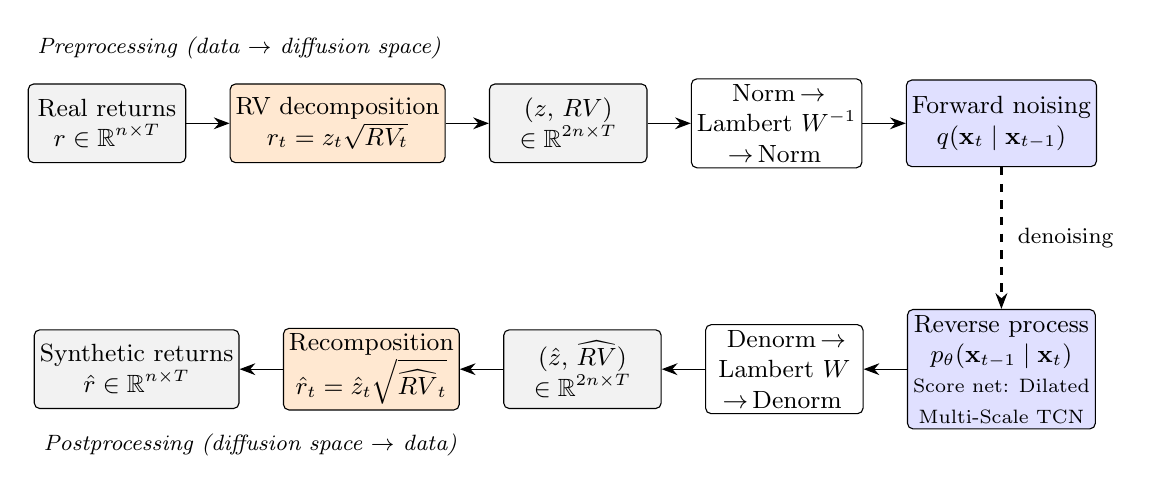
\begin{tikzpicture}[
  font=\small,
  >={Stealth[length=2mm]},
  node distance=0.55cm,
  data/.style ={draw, rounded corners=2pt, fill=gray!10,  minimum height=1.0cm, minimum width=2.0cm, align=center, inner sep=2pt},
  op/.style   ={draw, rounded corners=2pt, fill=white,    minimum height=1.0cm, minimum width=2.0cm, align=center, inner sep=2pt},
  dec/.style  ={draw, rounded corners=2pt, fill=orange!18, minimum height=1.0cm, minimum width=2.1cm, align=center, inner sep=2pt},
  diff/.style ={draw, rounded corners=2pt, fill=blue!12,  minimum height=1.1cm, minimum width=2.2cm, align=center, inner sep=2pt},
]

% --- Top row: forward pipeline ---
\node[data] (r)    {Real returns \\ $r \in \mathbb{R}^{n\times T}$};
\node[dec, right=of r]    (rvd)  {RV decomposition \\ $r_t = z_t\sqrt{RV_t}$};
\node[data,right=of rvd]  (z2n)  {$(z,\, RV)$ \\ $\in \mathbb{R}^{2n\times T}$};
\node[op,  right=of z2n]  (lw1)  {Norm $\!\to\!$ \\ Lambert $W^{-1}$ \\ $\!\to\!$ Norm};
\node[diff,right=of lw1]  (qfwd) {Forward noising \\ $q(\mathbf{x}_t \mid \mathbf{x}_{t-1})$};

\draw[->] (r)    -- (rvd);
\draw[->] (rvd)  -- (z2n);
\draw[->] (z2n)  -- (lw1);
\draw[->] (lw1)  -- (qfwd);

% --- Bottom row: reverse pipeline ---
\node[diff, below=1.8cm of qfwd] (rev) {Reverse process \\ $p_\theta(\mathbf{x}_{t-1} \mid \mathbf{x}_t)$ \\ \scriptsize Score net: Dilated \\ \scriptsize Multi-Scale TCN};
\node[op,   left=of rev]   (lw2)    {Denorm $\!\to\!$ \\ Lambert $W$ \\ $\!\to\!$ Denorm};
\node[data, left=of lw2]   (z2nhat) {$(\hat z,\, \widehat{RV})$ \\ $\in \mathbb{R}^{2n\times T}$};
\node[dec,  left=of z2nhat](rec)    {Recomposition \\ $\hat r_t = \hat z_t\sqrt{\widehat{RV}_t}$};
\node[data, left=of rec]   (rhat)   {Synthetic returns \\ $\hat r \in \mathbb{R}^{n\times T}$};

\draw[->] (rev)    -- (lw2);
\draw[->] (lw2)    -- (z2nhat);
\draw[->] (z2nhat) -- (rec);
\draw[->] (rec)    -- (rhat);

% --- Connector ---
\draw[->, very thick, dashed] (qfwd.south) -- node[right=2pt, midway]{\footnotesize denoising} (rev.north);

% --- Group labels ---
\node[font=\footnotesize\itshape, anchor=west] at ([yshift=0.45cm]r.north west) {Preprocessing (data $\to$ diffusion space)};
\node[font=\footnotesize\itshape, anchor=west] at ([yshift=-0.45cm]rhat.south west) {Postprocessing (diffusion space $\to$ data)};

\end{tikzpicture}

\caption{Overall architecture of QuantDiffusion.}
\label{fig:architecture}
\end{figure*}



\section{NOISE STRUCTURE}
Because the series is decomposed into a bulk component and a tail component, we adopt the $\ell_1$ loss as the training objective; empirically, it performs better than the $\ell_2$ loss in our setting.

We denote by $\tau$ the temperature parameter, which controls the shape of nonlinear noise schedules (such as cosine or sigmoid schedules) and determines the steepness of the curve as well as the speed of noise injection. The minimum noise variance $\beta_{\min}$ (i.e., $\beta_1$) is the smallest amount of noise (variance) injected into the original data at the first diffusion step. The maximum noise variance $\beta_{\max}$ (i.e., $\beta_T$) is the largest amount of noise (variance) injected at the final diffusion step to fully collapse the data into pure noise.

\subsection{Noise Process}
Conventional Gaussian based diffusion models exhibit a fundamental limitation in that probability density tends to concentrate on a narrow spherical shell in high dimensional space, which makes it difficult to capture extreme and rare tail events. To overcome this limitation, heavy tailed diffusion models such as t-EDM and t-Flow~\cite{noiseprocessPandey24}, which adopt a multivariate Student-$t$ distribution as the prior noise distribution, accurately capture the tail region of the data distribution and substantially improve generation accuracy for extreme phenomena on the high resolution weather benchmark (HRRR) relative to Gaussian counterparts. Building on these findings, we adopt the Student-$t$ distribution as the prior noise distribution.

\subsection{Noise Schedule}
The Adaptive Noise schedule for Time series diffusion models (ANT) proposed by Lee et al.~\cite{ANTLee24} is a data adaptive noise scheduling technique designed to overcome the performance degradation that arises when noise schedules borrowed from other domains are applied indiscriminately to time series diffusion models. The work leverages the IAAT statistic, which measures the non stationarity intrinsic to time series data, and evaluates schedules holistically against three key criteria: (i) whether the non stationarity of the data decreases linearly and uniformly ($\lambda_{\mathrm{linear}}$); (ii) whether the data collapses into fully random noise at the final step ($\lambda_{\mathrm{noise}}$); and (iii) whether the number of diffusion steps $T$ is sufficient ($\lambda_{\mathrm{step}}$). The ANT algorithm is practical in that it can search for the optimal schedule offline, using only lightweight computations and without any additional model training. Guided by these considerations and by the desire for finer learning in the early stages of training, we adopt the cosine scheduler, and based on the ANT score we select $\tau = 1.5$, $\beta_{\min} = 1 \times 10^{-5}$, $\beta_{\max} = 0.5$, and a total of $T = 75$ diffusion time steps. The model is trained for $45$ epochs under this configuration.
% \begin{figure}
%     \centering
%     \includegraphics[width=0.75\linewidth]{figure1_ANT.png}
%     \caption{ANT score analysis under the selected cosine schedule ($\tau=1.5$, $\beta_{\min}=10^{-5}$, $\beta_{\max}=0.5$, $T=75$). The scaled IAAT trajectory (solid) is compared against the ideal linear decay (dashed); the shaded region quantifies their deviation, yielding an ANT score of $0.1930$.}
%     \label{fig:placeholder}
% \end{figure}

\section{EXPERIMENTS}

We examine how QuantDiffusion behaves on multivariate financial return data, both in terms of statistical fidelity and downstream risk performance. The goal is twofold: to verify that the generated series reproduce the stylized facts and inter asset dependence of real markets, and to assess whether the proposed design translates into measurable improvements in portfolio level tail risk estimation.

QuantDiffusion is benchmarked against three state of the art baselines that span the two dominant paradigms in the recent literature. Two are GAN based: QuantGAN, which couples a temporal convolutional backbone with the Lambert$~W$ transform, and Tail-GAN, which targets tail risk fidelity through a quantile based adversarial objective. The third, Diffusion-TS, is a transformer based denoising diffusion model with a trend seasonality decomposition. Together they cover temporal convolutional architectures, tail oriented adversarial training, and transformer based diffusion, providing a representative cross section of the current state of the art.

To assess statistical fidelity we report metrics targeting inter variable dependence, marginal distributional features, and temporal dependence:

\begin{itemize}
    \item \textbf{Cross correlation function (CCF)}: For variables $i \ne j$, $\rho_\tau(X_i, X_j) = \mathrm{Corr}(x_{i,t}, x_{j,t+\tau})$. We report the average absolute discrepancy between real and synthetic CCFs across all pairs and lags up to $\tau_{\max} = 10$:
    \begin{equation}
        \mathrm{CCF}(\tau_{\max}) = \sum_{\tau=0}^{\tau_{\max}}
        \bigl|\rho_\tau(X_i,X_j) - \rho_\tau(\widehat{X}_i,\widehat{X}_j)\bigr|.
    \end{equation}

    \item \textbf{Kolmogorov--Smirnov statistic}~\cite{KS-test}: $\mathrm{KS}(p,q) = \sup_{x} |F_p(x) - F_q(x)|$, where $F_p, F_q$ are the empirical CDFs.
    
    \item \textbf{Skewness/kurtosis difference}: For each variable $i$, $\mathrm{Skew} = |S(X_i) - S(\widehat{X}_i)|$ and $\mathrm{Kurt} = |K(X_i) - K(\widehat{X}_i)|$, averaged across variables.

    \item \textbf{Linear / non linear ACF}: For $g(\cdot)$,
    \begin{equation}
        \mathrm{ACF}(g) = \sum_{\tau=1}^{\tau_{\max}}
        \bigl(\rho_\tau(g(X_i)) - \rho_\tau(g(\widehat{X}_i))\bigr)^2,
    \end{equation}
    with $g(x)=x$ for linear and $g(x)=x^2$ or $|x|$ for non linear dependence; $\tau_{\max} = 40$.

    \item \textbf{Leverage effect}: With $\mathrm{Lev}_\tau(X_i) = \mathrm{Corr}(x_{i,t}, x_{i,t+\tau}^2)$,
    \begin{equation}
        \mathrm{Leverage\ Effect} = \sum_{\tau=1}^{\tau_{\max}}
        \bigl(\mathrm{Lev}_\tau(X_i) - \mathrm{Lev}_\tau(\widehat{X}_i)\bigr)^2, \quad \tau_{\max}=40.
    \end{equation}
\end{itemize}

Beyond statistical fidelity, faithful capture of extreme losses is essential for risk sensitive applications. Following Tail-GAN~\cite{Cont26}, we evaluate the alignment of portfolio level \emph{Value at Risk} (VaR) and \emph{Expected Shortfall} (ES) under real and synthetic scenarios. P\&L values are obtained by exponentiating cumulative sums of generated log returns with an initial price of $100$. For portfolio strategy $u$ inducing CDF $F_p^u$ (real) or $F_q^u$ (synthetic):
{\footnotesize
\begin{align}
    \mathrm{VaR}_\alpha^u(p) &= \inf\bigl\{ x : F_p^u(x) \ge \alpha \bigr\}, &
    \mathrm{ES}_\alpha^u(p) &= \tfrac{1}{\alpha}\!\int_0^\alpha \mathrm{VaR}_\beta^u(p)\,d\beta,
\end{align}

\begin{equation}
    \mathrm{RE}^{\mathrm{VaR}}_\alpha(u)
    =
    \frac{
    |\mathrm{VaR}_\alpha^u(q)-\mathrm{VaR}_\alpha^u(p)|
    }{
    |\mathrm{VaR}_\alpha^u(p)|
    },
    \qquad
    \mathrm{RE}^{\mathrm{ES}}_\alpha(u)
    =
    \frac{
    |\mathrm{ES}_\alpha^u(q)-\mathrm{ES}_\alpha^u(p)|
    }{
    |\mathrm{ES}_\alpha^u(p)|
    }.
\end{equation}
}
Unlike conventional evaluations restricted to the terminal timestep $T$, we compute these errors at all intermediate $t \le T$ to test whether the generated scenarios reproduce the \emph{evolution} of risk exposure rather than its endpoint alone.

\subsection{Data}

The empirical analysis uses daily log returns from adjusted closing prices of six assets: the DJIA, the Nasdaq Composite, JP Morgan (JPM) equity, the Hang Seng Index (HSI), Gold futures, and WTI crude oil futures. The set is constructed to reflect a diversified cross section of major markets and to expose a range of dependence structures---highly correlated assets (DJIA and Nasdaq) alongside more weakly correlated or diversifying ones (HSI, Gold)---so that marginal fidelity and inter asset dependence can be evaluated jointly.

Price data are obtained from the Center for Research on Security Prices (CRSP) and span January~1,~2001 through December~31,~2025. A sliding window strategy with a $256$ day window yields approximately $6{,}000$ samples in $\mathbb{R}^{6 \times 256}$. To preserve temporal ordering and avoid look ahead bias, the earliest $70\%$ are used for training and the remaining $30\%$ for out of sample evaluation.

\subsection{Results}

Table~\ref{table:statistical_fidelity_combined} reports statistical fidelity metrics covering inter asset dependence, marginal distributions, and temporal structure. Out of the seventeen fidelity metrics, QuantDiffusion attains the best score on twelve and is among the top two on fifteen, the exceptions being confined to skewness, and its standard deviations across seeds are typically among the smallest of all models.

\begin{table*}[htbp]
\centering
\caption{Statistical fidelity comparison across dependence, marginal distribution, and temporal structure metrics. Best in \textbf{bold}, second best \underline{underlined}; lower is better.}
\label{table:statistical_fidelity_combined}

\scriptsize
\setlength{\tabcolsep}{3pt}
\renewcommand{\arraystretch}{0.9}

\begin{adjustbox}{max width=\textwidth}
\begin{tabular}{l|cccc}
\toprule
\textbf{Metric} & \textbf{TailGAN} & \textbf{QuantGAN} & \textbf{Diffusion-TS} & \textbf{QuantDiffusion} \\
\midrule
CCF($\tau = 0$)
& 0.1987 $\pm$ 0.0002
& 0.0968 $\pm$ 0.0005
& \textbf{0.0533} $\pm$ 0.0010
& \underline{0.0572} $\pm$ 0.0007 \\
CCF($\tau > 0$)
& 0.0666 $\pm$ 0.0001
& 0.0569 $\pm$ 0.0002
& \underline{0.0367} $\pm$ 0.0002
& \textbf{0.0341} $\pm$ 0.0002 \\
\midrule
KS(1)
& 0.1820 $\pm$ 0.0002
& \underline{0.0402} $\pm$ 0.0001
& 0.0948 $\pm$ 0.0006
& \textbf{0.0375} $\pm$ 0.0000 \\
KS(5)
& 0.1759 $\pm$ 0.0003
& \underline{0.0529} $\pm$ 0.0003
& 0.1141 $\pm$ 0.0005
& \textbf{0.0418} $\pm$ 0.0003 \\
KS(20)
& 0.1823 $\pm$ 0.0006
& \underline{0.0785} $\pm$ 0.0006
& 0.1335 $\pm$ 0.0005
& \textbf{0.0530} $\pm$ 0.0004 \\
KS(100)
& 0.2425 $\pm$ 0.0017
& \underline{0.1404} $\pm$ 0.0016
& 0.1912 $\pm$ 0.0011
& \textbf{0.1403} $\pm$ 0.0024 \\
\midrule
Skew(1)
& 0.2245 $\pm$ 0.0017
& 0.4560 $\pm$ 0.0135
& \textbf{0.1507} $\pm$ 0.0039
& \underline{0.1582} $\pm$ 0.0037 \\
Skew(5)
& \underline{0.2683} $\pm$ 0.0020
& 0.3424 $\pm$ 0.0083
& \textbf{0.1436} $\pm$ 0.0050
& 0.3335 $\pm$ 0.0073 \\
Skew(20)
& 0.2760 $\pm$ 0.0020
& \underline{0.2277} $\pm$ 0.0070
& \textbf{0.2043} $\pm$ 0.0018
& 0.3380 $\pm$ 0.0046 \\
Skew(100)
& 0.1262 $\pm$ 0.0067
& \textbf{0.0853} $\pm$ 0.0063
& \underline{0.0955} $\pm$ 0.0025
& 0.1199 $\pm$ 0.0058 \\
\midrule
Kurt(1)
& 4.2878 $\pm$ 0.0017
& 5.1508 $\pm$ 0.2507
& \underline{2.9343} $\pm$ 0.0070
& \textbf{0.7942} $\pm$ 0.0515 \\
Kurt(5)
& 1.6039 $\pm$ 0.0029
& \underline{0.9097} $\pm$ 0.0589
& 1.0401 $\pm$ 0.0168
& \textbf{0.8688} $\pm$ 0.0288 \\
Kurt(20)
& 0.7140 $\pm$ 0.0033
& \underline{0.5001} $\pm$ 0.0087
& 0.6869 $\pm$ 0.0071
& \textbf{0.2287} $\pm$ 0.0101 \\
Kurt(100)
& 0.2637 $\pm$ 0.0055
& 0.2678 $\pm$ 0.0109
& \underline{0.2555} $\pm$ 0.0077
& \textbf{0.2037} $\pm$ 0.0122 \\
\midrule
ACF($x$)
& 0.0010 $\pm$ 0.0000
& 0.0012 $\pm$ 0.0000
& \textbf{0.0007} $\pm$ 0.0000
& \underline{0.0008} $\pm$ 0.0000 \\
ACF($|x|$)
& 0.0051 $\pm$ 0.0000
& \underline{0.0038} $\pm$ 0.0000
& 0.0041 $\pm$ 0.0000
& \textbf{0.0015} $\pm$ 0.0001 \\
ACF($x^2$)
& 0.0030 $\pm$ 0.0000
& \underline{0.0023} $\pm$ 0.0000
& 0.0023 $\pm$ 0.0000
& \textbf{0.0009} $\pm$ 0.0000 \\
\midrule
Lev. Effect
& 0.0016 $\pm$ 0.0000
& \underline{0.0011} $\pm$ 0.0000
& 0.0012 $\pm$ 0.0000
& \textbf{0.0007} $\pm$ 0.0000 \\
\bottomrule
\end{tabular}
\end{adjustbox}
\end{table*}


\begin{table*}[htbp]
\centering
\caption{Ablation study: statistical fidelity of QuantDiffusion (Baseline = full model) when each key component is removed (RV decomposition, Lambert-W Gaussianization, ModernTCN backbone). Best in \textbf{bold}, second best \underline{underlined}; lower is better.}
\label{table:ablation_fidelity}

\scriptsize
\setlength{\tabcolsep}{3pt}
\renewcommand{\arraystretch}{0.9}

\begin{adjustbox}{max width=\textwidth}
\begin{tabular}{l|cccc}
\toprule
\textbf{Metric} & \textbf{Baseline} & \textbf{w/o RV Decomp.} & \textbf{w/o LambertW} & \textbf{w/o ModernTCN} \\
\midrule
CCF($\tau = 0$)
& 0.0572 $\pm$ 0.0007
& \underline{0.0524} $\pm$ 0.0005
& 0.0709 $\pm$ 0.0003
& \textbf{0.0390} $\pm$ 0.0005 \\
CCF($\tau > 0$)
& \underline{0.0341} $\pm$ 0.0002
& 0.0342 $\pm$ 0.0001
& 0.0420 $\pm$ 0.0001
& \textbf{0.0276} $\pm$ 0.0001 \\
\midrule
KS(1)
& 0.0375 $\pm$ 0.0000
& \textbf{0.0328} $\pm$ 0.0002
& 0.0379 $\pm$ 0.0002
& \underline{0.0342} $\pm$ 0.0002 \\
KS(5)
& \textbf{0.0418} $\pm$ 0.0003
& 0.0446 $\pm$ 0.0003
& 0.0437 $\pm$ 0.0003
& \underline{0.0424} $\pm$ 0.0002 \\
KS(20)
& \textbf{0.0530} $\pm$ 0.0004
& 0.0647 $\pm$ 0.0005
& \underline{0.0622} $\pm$ 0.0006
& 0.0660 $\pm$ 0.0005 \\
KS(100)
& 0.1403 $\pm$ 0.0024
& \textbf{0.1300} $\pm$ 0.0016
& 0.1722 $\pm$ 0.0020
& \underline{0.1399} $\pm$ 0.0018 \\
\midrule
Skew(1)
& 0.1582 $\pm$ 0.0037
& \textbf{0.0845} $\pm$ 0.0062
& \underline{0.1520} $\pm$ 0.0051
& 0.1920 $\pm$ 0.0054 \\
Skew(5)
& 0.3335 $\pm$ 0.0073
& \underline{0.2032} $\pm$ 0.0133
& 0.3393 $\pm$ 0.0030
& \textbf{0.1076} $\pm$ 0.0024 \\
Skew(20)
& 0.3380 $\pm$ 0.0046
& \underline{0.2143} $\pm$ 0.0074
& 0.3579 $\pm$ 0.0042
& \textbf{0.1616} $\pm$ 0.0076 \\
Skew(100)
& 0.1199 $\pm$ 0.0058
& \textbf{0.0818} $\pm$ 0.0020
& 0.1155 $\pm$ 0.0033
& \underline{0.0893} $\pm$ 0.0037 \\
\midrule
Kurt(1)
& \underline{0.7942} $\pm$ 0.0515
& 1.6739 $\pm$ 0.0490
& 0.8877 $\pm$ 0.0305
& \textbf{0.7817} $\pm$ 0.0375 \\
Kurt(5)
& 0.8688 $\pm$ 0.0288
& \underline{0.4753} $\pm$ 0.0131
& 0.9116 $\pm$ 0.0182
& \textbf{0.4427} $\pm$ 0.0106 \\
Kurt(20)
& \textbf{0.2287} $\pm$ 0.0101
& 0.5363 $\pm$ 0.0065
& \underline{0.2997} $\pm$ 0.0234
& 0.3646 $\pm$ 0.0130 \\
Kurt(100)
& \underline{0.2037} $\pm$ 0.0122
& 0.2313 $\pm$ 0.0040
& \textbf{0.1690} $\pm$ 0.0089
& 0.2536 $\pm$ 0.0077 \\
\midrule
ACF($x$)
& \underline{0.0008} $\pm$ 0.0000
& 0.0008 $\pm$ 0.0000
& 0.0009 $\pm$ 0.0000
& \textbf{0.0007} $\pm$ 0.0000 \\
ACF($|x|$)
& \textbf{0.0015} $\pm$ 0.0001
& 0.0039 $\pm$ 0.0000
& 0.0021 $\pm$ 0.0001
& \underline{0.0018} $\pm$ 0.0000 \\
ACF($x^2$)
& \textbf{0.0009} $\pm$ 0.0000
& 0.0024 $\pm$ 0.0000
& \underline{0.0012} $\pm$ 0.0000
& 0.0012 $\pm$ 0.0000 \\
\midrule
Lev. Effect
& \textbf{0.0007} $\pm$ 0.0000
& 0.0010 $\pm$ 0.0000
& \underline{0.0009} $\pm$ 0.0000
& 0.0010 $\pm$ 0.0000 \\
\bottomrule
\end{tabular}
\end{adjustbox}
\end{table*}

\paragraph{Inter asset dependence.}
On contemporaneous cross correlation, CCF($\tau=0$), Diffusion-TS attains the lowest error at $0.0533$, with QuantDiffusion second at $0.0572$; the two separate clearly from QuantGAN ($0.0968$) and Tail-GAN ($0.1987$). On the lagged metric CCF($\tau>0$), the ordering changes and QuantDiffusion ranks first at $0.0341$, ahead of Diffusion-TS at $0.0367$. This pattern is consistent with the design. Diffusing on the joint representation $(z_t, RV_t)$ lets the shock component $z_t$ carry the contemporaneous comovement while $RV_t$ transmits the cross asset comovement of risk that governs lagged dependence, which explains why QuantDiffusion is strongest precisely on the lagged structure. Diffusion-TS, which lacks an explicit volatility channel, recovers the contemporaneous correlation accurately but sustains it less well across lags.

\paragraph{Marginal distributions.}
QuantDiffusion achieves the lowest KS statistic at every horizon $h \in \{1, 5, 20, 100\}$, with QuantGAN second throughout; at $h = 100$ the margin is negligible ($0.1403$ versus $0.1404$), whereas at the shorter horizons the lead is pronounced. Tail-GAN is the weakest at every horizon, and Diffusion-TS trails the GAN baselines at the shorter horizons. The kurtosis row is the most consequential for risk, since kurtosis is a primary indicator of fat tailed behavior. QuantDiffusion attains the lowest kurtosis error at every horizon, and the advantage is most striking at $h = 1$ ($0.7942$), less than a third of the next best model (Diffusion-TS at $2.9343$) and less than a fifth of QuantGAN ($5.1508$). This is the clearest single piece of evidence in the table that the realized volatility decomposition reinstates the fat tailed behavior of returns. The skewness metrics are the sole weakness, with QuantDiffusion second at $h = 1$, last at $h \in \{5, 20\}$, and third at $h = 100$. This is a structural consequence of the decomposition, since dividing returns by $\sqrt{RV_t}$ renders the shock $z_t$ approximately symmetric, so the sample skewness of the reconstructed series depends on the joint $(z_t, RV_t)$ dynamics rather than on a marginal moment that the diffusion model targets directly. The ablation in Table~\ref{table:ablation_fidelity} corroborates this reading, since removing the RV decomposition improves skewness while degrading the volatility clustering metrics.

\paragraph{Temporal and nonlinear dependence.}
The most decisive evidence for the SDE aware design lies in the nonlinear autocorrelation metrics. QuantDiffusion attains $0.0015$ on $\mathrm{ACF}(|x|)$ and $0.0009$ on $\mathrm{ACF}(x^{2})$, against $0.0041$ and $0.0023$ for Diffusion-TS, errors between two and three times larger for the transformer based diffusion model, and it likewise leads on the leverage effect ($0.0007$ versus $0.0012$ for Diffusion-TS); on all three metrics QuantGAN is second and QuantDiffusion improves on it by a clear margin (a factor of about $2.5$ on the two absolute and squared autocorrelations and about $1.6$ on the leverage effect). On the linear $\mathrm{ACF}(x)$ all models are effectively tied near the noise floor, between $0.0007$ and $0.0012$. Despite being a state of the art diffusion model, Diffusion-TS fails to reproduce the persistence in $|x|$ and $x^{2}$ that drives volatility clustering. This is consistent with the argument of Section~3, namely that a diffusion model which ingests raw returns cannot separate Brownian volatility fluctuations from the injected diffusion noise, whereas extracting the volatility component beforehand frees the score network to learn genuine nonlinear temporal structure.

\begin{table*}[htbp]
\centering
\caption{Portfolio risk fidelity: relative error of VaR and ES (averaged over the four trading strategies) between synthetic and historical data. Best in \textbf{bold}, second best \underline{underlined}; lower is better.}
\label{table:portfolio_risk}

\scriptsize
\setlength{\tabcolsep}{3pt}
\renewcommand{\arraystretch}{0.9}

\begin{adjustbox}{max width=\textwidth}
\begin{tabular}{l|cccc}
\toprule
\textbf{Metric} & \textbf{TailGAN} & \textbf{QuantGAN} & \textbf{Diffusion-TS} & \textbf{QuantDiffusion} \\
\midrule
$\text{RE}_{\text{VaR}}(0.05)$
& 0.5343 $\pm$ 0.0064
& \underline{0.5340} $\pm$ 0.0112
& 0.5684 $\pm$ 0.0048
& \textbf{0.3514} $\pm$ 0.0054 \\
$\text{RE}_{\text{VaR}}(0.025)$
& 0.5278 $\pm$ 0.0061
& 0.5951 $\pm$ 0.0131
& \underline{0.4797} $\pm$ 0.0198
& \textbf{0.3259} $\pm$ 0.0026 \\
$\text{RE}_{\text{VaR}}(0.01)$
& 0.5605 $\pm$ 0.0065
& 0.6745 $\pm$ 0.0158
& \underline{0.4110} $\pm$ 0.0180
& \textbf{0.3351} $\pm$ 0.0034 \\
\midrule
$\text{RE}_{\text{ES}}(0.05)$
& 0.5429 $\pm$ 0.0091
& 0.6346 $\pm$ 0.0213
& \underline{0.4527} $\pm$ 0.0163
& \textbf{0.3276} $\pm$ 0.0023 \\
$\text{RE}_{\text{ES}}(0.025)$
& 0.5842 $\pm$ 0.0109
& 0.7237 $\pm$ 0.0363
& \underline{0.3995} $\pm$ 0.0189
& \textbf{0.3277} $\pm$ 0.0038 \\
$\text{RE}_{\text{ES}}(0.01)$
& 0.6572 $\pm$ 0.0190
& 0.8619 $\pm$ 0.0753
& \underline{0.3622} $\pm$ 0.0062
& \textbf{0.3388} $\pm$ 0.0104 \\
\bottomrule
\end{tabular}
\end{adjustbox}
\end{table*}

\paragraph{Portfolio level Value at Risk}

Table~\ref{table:portfolio_risk} reports the average relative error of portfolio level Value at Risk over the four trading strategies at three confidence levels. QuantDiffusion attains the smallest error at every level, with $0.3514$, $0.3259$, and $0.3351$ at $\alpha \in \{0.05, 0.025, 0.01\}$, and its error is essentially flat across confidence levels rather than deteriorating deeper in the tail. The second best model varies by level, being QuantGAN at $\alpha = 0.05$ and Diffusion-TS at the two tighter levels, yet the margin is substantial throughout: relative to the second best, QuantDiffusion reduces the error by $34.2\%$ at $\alpha = 0.05$, $32.1\%$ at $\alpha = 0.025$, and $18.5\%$ at $\alpha = 0.01$. The GAN baselines, whose VaR errors range from roughly $0.53$ to $0.67$ and worsen as $\alpha$ tightens, illustrate that accurate unconditional statistics alone are not sufficient for tail quantile fidelity. QuantDiffusion also exhibits low dispersion across seeds, a practically relevant property for risk pipelines that rerun the generator across many scenarios.

\begin{table*}[htbp]
\centering
\caption{Ablation study on portfolio risk fidelity: relative error of VaR and ES (averaged over the four trading strategies) when each key component of QuantDiffusion (Baseline = full model) is removed. Best in \textbf{bold}, second best \underline{underlined}; lower is better.}
\label{table:ablation_portfolio_risk}

\scriptsize
\setlength{\tabcolsep}{3pt}
\renewcommand{\arraystretch}{0.9}

\begin{adjustbox}{max width=\textwidth}
\begin{tabular}{l|cccc}
\toprule
\textbf{Metric} & \textbf{Baseline} & \textbf{w/o RV Decomp.} & \textbf{w/o LambertW} & \textbf{w/o ModernTCN} \\
\midrule
$\text{RE}_{\text{VaR}}(0.05)$
& \textbf{0.3514} $\pm$ 0.0054
& 0.6559 $\pm$ 0.0040
& \underline{0.3814} $\pm$ 0.0009
& 0.4055 $\pm$ 0.0063 \\
$\text{RE}_{\text{VaR}}(0.025)$
& \textbf{0.3259} $\pm$ 0.0026
& 0.6278 $\pm$ 0.0042
& \underline{0.3543} $\pm$ 0.0012
& 0.3716 $\pm$ 0.0052 \\
$\text{RE}_{\text{VaR}}(0.01)$
& \textbf{0.3351} $\pm$ 0.0034
& 0.6131 $\pm$ 0.0029
& \underline{0.3582} $\pm$ 0.0021
& 0.3676 $\pm$ 0.0039 \\
\midrule
$\text{RE}_{\text{ES}}(0.05)$
& \textbf{0.3276} $\pm$ 0.0023
& 0.6216 $\pm$ 0.0031
& \underline{0.3546} $\pm$ 0.0013
& 0.3696 $\pm$ 0.0046 \\
$\text{RE}_{\text{ES}}(0.025)$
& \textbf{0.3277} $\pm$ 0.0038
& 0.6045 $\pm$ 0.0022
& \underline{0.3490} $\pm$ 0.0014
& 0.3565 $\pm$ 0.0035 \\
$\text{RE}_{\text{ES}}(0.01)$
& \textbf{0.3388} $\pm$ 0.0104
& 0.5797 $\pm$ 0.0028
& 0.3534 $\pm$ 0.0043
& \underline{0.3453} $\pm$ 0.0036 \\
\bottomrule
\end{tabular}
\end{adjustbox}
\end{table*}

\paragraph{Portfolio level Expected Shortfall}

Because VaR alone does not capture the magnitude of losses beyond its threshold, we complement the analysis above with the Expected Shortfall errors, the more stringent tail risk measure, reported in the lower panel of Table~\ref{table:portfolio_risk}. QuantDiffusion is again uniformly best, with relative errors of $0.3276$, $0.3277$, and $0.3388$ at $\alpha \in \{0.05, 0.025, 0.01\}$. The second best model at every level is Diffusion-TS ($0.4527$, $0.3995$, $0.3622$), so QuantDiffusion improves upon it by $27.6\%$, $18.0\%$, and $6.5\%$ respectively, while its lead over the GAN baselines, whose errors reach as high as $0.8619$, is larger still. A notable qualitative difference is that the error of Diffusion-TS decreases as $\alpha$ tightens, opposite to the near constant profile of QuantDiffusion. We read this as evidence that the transformer backbone produces an over dispersed profit and loss distribution whose bulk diverges from the empirical one more strongly than its deep tail, so that the averaging region of ES, pushed further into the tail, coincides with a range where the over dispersion partially offsets the empirical mass. Because ES is structurally more sensitive than VaR to the entire shape of the tail, the persistence of QuantDiffusion's advantage under this measure indicates that the realized volatility decomposition recovers the tail distribution rather than a single tail quantile. Taken together, Table~\ref{table:portfolio_risk} shows that QuantDiffusion produces scenarios that are most reliable precisely in the regime where reliability is hardest to obtain, and that adopting a state of the art diffusion architecture without an explicit financial process prior, as in Diffusion-TS, is insufficient to deliver this property.

\subsection{Ablation Study}

Tables~\ref{table:ablation_fidelity} and~\ref{table:ablation_portfolio_risk} isolate the contribution of each component by removing it from the full model. The clearest overall effect is that the full configuration is strongest on the metrics that describe how volatility clusters and evolves over time, that is $\mathrm{ACF}(|x|)$, $\mathrm{ACF}(x^{2})$, and the leverage effect, and on the portfolio level tail risk measures. Each component therefore contributes primarily to temporal structure and to tail risk rather than to the shape of any individual marginal moment. Examining the components one at a time makes their distinct roles explicit.

\paragraph{Realized volatility decomposition.}
Removing the RV decomposition all but eliminates the model's ability to reproduce volatility clustering: $\mathrm{ACF}(|x|)$ rises from $0.0015$ to $0.0039$ and $\mathrm{ACF}(x^{2})$ from $0.0009$ to $0.0024$, and the portfolio tail risk errors become the worst in the ablation, between $0.58$ and $0.66$ across all confidence levels. This follows directly from the fact that, without the decomposition, the model can no longer separate a residual shock from a volatility magnitude and generate the two processes independently. A revealing counterpoint is that skewness improves markedly, with the variant attaining the best skewness at $h = 1$ and $h = 100$. The decomposition is designed to orthogonalize the shock $z_t$ and the scale $\sqrt{RV_t}$, and dividing returns by the scale compresses large negative shocks toward the center, so that $z_t$ becomes nearly symmetric. Because generation then draws $z_t$ and $\sqrt{RV_t}$ almost independently and multiplies them, the association between negative returns and elevated volatility that produces skewness is not reconstructed, and the output is too symmetric. When the decomposition is removed, the model instead learns the raw returns directly and retains their skewness. The RV decomposition thus embodies a trade off in which a portion of marginal skewness is exchanged for a substantial gain in volatility clustering and tail risk fidelity.

\paragraph{Lambert-W transform.}
The Lambert-W transform draws the far reaching extreme tail toward the center and renders the data closer to Gaussian, and it contributes unexpectedly to the modeling of volatility clustering. Removing it degrades $\mathrm{ACF}(|x|)$ from $0.0015$ to $0.0021$, $\mathrm{ACF}(x^{2})$ from $0.0009$ to $0.0012$, and Kurt($1$) from $0.7942$ to $0.8877$. We attribute this to the fact that, even after the RV decomposition, extreme values remain in the residual, and the model expends learning capacity fitting these outliers, leaving less capacity for the temporal structure captured by the autocorrelation functions. This observation motivates a change in the logical ordering of our argument. Rather than assuming the SVJD process first and introducing the Lambert-W transform to suit it, we start from the empirical finding that separating out the extreme mass improves kurtosis and clustering together, infer that real financial series contain a jump component that impedes the learning of the tail, and conclude that a specification which isolates such jumps is appropriate. Under this ordering the SVJD model is not an arbitrary prior imposed in order to justify the transform, but a specification that the empirical results support a posteriori as a suitable description of real financial time series.

\paragraph{ModernTCN backbone.}
A conventional temporal convolutional network cannot secure a global receptive field by increasing depth alone, since additional layers raise computation while the effective receptive field grows only sub linearly, in contrast to architectures with globally connected receptive fields such as Transformers. The ModernTCN backbone instead combines large and small kernels so as to capture wide temporal structure at once, which is reflected in its accurate autocorrelation: the full model improves on the variant without ModernTCN on both $\mathrm{ACF}(|x|)$ ($0.0015$ versus $0.0018$) and $\mathrm{ACF}(x^{2})$ ($0.0009$ versus $0.0012$). That ModernTCN reproduces the autocorrelation faithfully can therefore be read as evidence that it genuinely attends to a broad temporal range. Its marginal accuracy is comparatively weaker, however, since the variant without ModernTCN is competitive or better on several KS, skewness, and kurtosis entries, which identifies improving marginal fidelity without sacrificing temporal structure as a direction for future work.

\paragraph{Tail risk.}
The portfolio ablation in Table~\ref{table:ablation_portfolio_risk} reinforces this picture. The full model attains the lowest relative error on all six VaR and ES entries, the variant without the RV decomposition is the worst by a large margin, and the variant without Lambert-W is closest to the full model. The RV decomposition is thus the dominant driver of tail risk fidelity, with the Lambert-W transform a secondary but consistent contributor.

\begin{figure}
    \centering
    \includegraphics[width=1\linewidth]{paper_hist_5day_asset2_JPM.png}
    \caption{Enter Caption}
    \label{fig:placeholder}
\end{figure}


\section{CONCLUSIONS AND FUTURE WORK}

We have proposed QuantDiffusion, a diffusion based generative framework for multivariate financial time series whose design choices are driven by the empirical requirements of financial generation and are subsequently grounded in an explicit stochastic process interpretation. By decomposing log returns via realized volatility and by treating the Lambert--$W$ transform as a $C^{2}$ invertible map on which It\^{o}'s lemma can be applied, the framework lifts what are typically regarded as preprocessing heuristics to operations that admit a precise meaning on the underlying SDE.

Empirically, this SDE aware design does not come at the cost of generative quality. Across equities, indices, and commodities, QuantDiffusion preserves cross asset dependence, the marginal return distributions across multiple horizons, and the nonlinear temporal dependence associated with volatility clustering at least as faithfully as the strongest baselines, while substantially reducing the estimation errors of portfolio level Value at Risk and Expected Shortfall.

Conventional deep generative approaches to financial time series tend to be opaque and weakly connected to the stochastic processes that financial theory has long formalized. The present work demonstrates that design choices which are first shown to improve tail and clustering fidelity can then be read consistently in terms of a concrete SDE specification, SVJD in our case, through It\^{o}'s lemma, so that the same construction simultaneously simplifies the learning target, improves tail risk fidelity, and restores a posteriori interpretability of the generated paths.

Several directions remain open. First, the realized volatility decomposition adopted here relies on a daily close to close realized variance, and we expect further gains from incorporating high frequency data, which would yield substantially more accurate realized volatility. Second, the SDE grounded design philosophy is not domain specific, and verifying QuantDiffusion's generation quality on other domains whose dynamics admit SDE representations would test the generality of the framework.

More broadly, we hope this work serves as a starting point for more active use of SDE based interpretation in deep generative models for financial time series, and that future work in this area remains consistent with the stochastic process foundations that the field has carefully built rather than treating them as legacy artifacts to be replaced.

\printbibliography

\end{document}
